\documentclass[11pt,a4paper]{article}
\usepackage[margin=2.1cm]{geometry}
\usepackage[T1]{fontenc}
\usepackage[utf8]{inputenc}
\usepackage{lmodern}
\usepackage{graphicx,booktabs,amsmath,array}
\usepackage{hyperref}
\usepackage{caption}
\usepackage{enumitem}
\hypersetup{colorlinks=true,linkcolor=blue,urlcolor=blue,citecolor=blue,pdftitle={Airbnb supply, prices and guest activity},pdfauthor={Project team}}
\setlength{\parindent}{0pt}
\setlength{\parskip}{6pt}
\setlength{\emergencystretch}{2em}
\newsavebox{\tablebox}
\setlength{\tabcolsep}{5pt}
\captionsetup{font=small,labelfont=bf}
\setlist{nosep,leftmargin=*}
\graphicspath{{../figures/}}
% Generated by scripts/build_report.py; do not edit numeric results manually.
\newcommand{\TotalListings}{177,860}
\newcommand{\TotalPriced}{154,226}
\newcommand{\TotalSpain}{38,001}
\newcommand{\MegaPooled}{50.2}
\newcommand{\MegaAverage}{51.6}
\newcommand{\SinglePooled}{28.3}
\newcommand{\MegaEntire}{72.8}
\newcommand{\SingleEntire}{71.9}
\newcommand{\PriceU}{155,985,046}
\newcommand{\PriceP}{5.17e-247}
\newcommand{\PriceSuperiority}{0.609}
\newcommand{\BcnShortN}{7,069}
\newcommand{\BcnShortPct}{46.2}
\newcommand{\MadShortN}{13,903}
\newcommand{\MadShortPct}{61.2}
\newcommand{\BcnEntireMonthly}{3,052}
\newcommand{\BcnEntireMonthlyN}{3,329}
\newcommand{\BcnPrivateMonthly}{1,157}
\newcommand{\BcnPrivateMonthlyN}{1,627}
\newcommand{\MadEntireMonthly}{3,023}
\newcommand{\MadEntireMonthlyN}{2,175}
\newcommand{\MadPrivateMonthly}{956}
\newcommand{\MadPrivateMonthlyN}{592}
\newcommand{\ModelN}{26,582}
\newcommand{\ModelRSq}{0.605}
\newcommand{\ModelAdjRSq}{0.605}
\newcommand{\ModelRank}{8}
\newcommand{\ModelCols}{8}
\newcommand{\ModelCondition}{59.2}
\newcommand{\CityPct}{-24.1}
\newcommand{\CityLow}{-25.2}
\newcommand{\CityHigh}{-22.9}
\newcommand{\BcnRho}{-0.059}
\newcommand{\BcnActivityN}{6,801}
\newcommand{\BcnEstablishedRho}{-0.116}
\newcommand{\MadRho}{-0.011}
\newcommand{\MadActivityN}{12,255}
\newcommand{\MadEstablishedRho}{-0.005}

\newcommand{\chart}[4][0.94]{\begin{figure}[htbp]\centering\includegraphics[width=#1\linewidth]{#2}\caption{#3}\label{#4}\end{figure}}
\newcommand{\resulttable}[3]{\begin{table}[htbp]\centering\small\sbox{\tablebox}{\input{report_tables/#1.tex}}\ifdim\wd\tablebox>\linewidth\resizebox{\linewidth}{!}{\usebox{\tablebox}}\else\usebox{\tablebox}\fi\caption{#2}\label{#3}\end{table}}
\newcommand{\question}[1]{\textbf{Research question.} #1}
\newcommand{\method}[1]{\textbf{Variables and method.} #1}
\newcommand{\finding}[1]{\textbf{Interpretation.} #1}
\begin{document}
\hypersetup{pageanchor=false}
\begin{titlepage}
\centering
\vspace*{1.6cm}
{\Large Universitat Rovira i Virgili\par}
{\large Sistemes d'Informaci\'o en les Organitzacions\par}
{\large Academic year 2026/27\par}
\vspace{1.7cm}
{\huge\bfseries Airbnb supply, prices\par and guest activity\par}
\vspace{0.5cm}
{\Large Six-city exploration with a focus\par on Barcelona and Madrid\par}
\vspace{1.2cm}
{\large Pr\`actica 1 -- El poder de les dades: El cas Airbnb\par}
\vspace{1cm}
\textbf{Team members: Kacper Lubecki, Sebastian Dawidowski, Marcel Kit\l{}owski}\par
25 October 2026\par
\vspace{1.2cm}
\begin{minipage}{0.88\textwidth}
\textbf{Abstract}\par
This project analyses \TotalListings{} Airbnb listing records from six city snapshots collected in June--July 2026. Four existing studies describe host-account concentration, price distributions, accommodation types and advertised minimum stays. Four additional studies focus on Barcelona and Madrid: the geography of entire homes accepting short stays, quoted costs of stays of about one month, a single descriptive price regression and the association between price and recent reviews.

The central distinction is between what the platform records and what these data cannot establish. Advertised prices, host minimums and reviews characterize the observed Airbnb market. They do not directly measure residential rents, household affordability, occupied nights, realized revenue or homes displaced from residential use. Reproducible notebooks, CSV result tables, code-generated figures and interactive HTML maps accompany this report.
\end{minipage}
\vfill
{\small Source of assignment requirements: the two PDFs supplied in \texttt{docs/}.\par}
\end{titlepage}
\hypersetup{pageanchor=true}

\tableofcontents
\clearpage
\section{Purpose, scope and housing context}
The aim is to describe the structure of Airbnb supply and pricing, then examine four focused questions for Barcelona and Madrid. We use six cities for the original comparisons: Barcelona--Los Angeles, Madrid--New York and Tokyo--Mexico City. These pairs organize the exploration; they do not constitute a policy experiment. The Spanish comparison has the practical advantage that both cities' prices are in euros.

Housing pressures motivate the choice of questions without becoming an outcome variable. Banco de Espa\~na's \emph{Annual Report 2023}, Chapter 4, describes increasing housing affordability difficulties, especially in urban and tourist areas, and discusses demand growth and limited supply responsiveness \cite{bde}. A June 2024 publication from Barcelona's housing consortium describes an announced plan to bring tourist flats back into residential use \cite{housing}. These publications provide historical policy context. We do not estimate the policy's effects or assume that its announced outcome has occurred.

\subsection{Eight substantive studies}
\begin{enumerate}
\item \textbf{02: Host economy.} Listing shares by host-account size, concentration, room composition and ratings.
\item \textbf{03: Price distribution.} Medians, means, dispersion, skewness, upper-tail observations and the Barcelona--Madrid comparison.
\item \textbf{04: Room type and price.} Conditional prices, relative median gaps and statistical comparisons.
\item \textbf{05: Rental model.} Minimum stays, availability and review proxies, calendar ranges, licence text and interactive geography.
\item \textbf{06: Short-stay geography.} Neighbourhood shares of entire homes with a 1--29-night minimum.
\item \textbf{07: Monthly-stay cost.} Valid 28--35-night quotations normalized to 30 nights.
\item \textbf{08: Price regression.} One OLS model of log price with basic listing characteristics and HC3 uncertainty estimates.
\item \textbf{09: Price and guest activity.} City-specific Spearman correlations and one established-listing sensitivity check.
\end{enumerate}
Notebook 01 is the initial audit and belongs to the methodology. It is not counted as a ninth substantive study. The study numbers therefore match the notebook filenames, with the rental-model study integrated as 05.

\subsection{What the project can establish}
The analyses quantify composition and associations in the repository snapshots. They can identify neighbourhoods where a particular type of Airbnb offer is relatively common, describe observed quotation costs and compare groups under explicit definitions. They cannot determine how many homes would be available to residents without Airbnb. No ordinary-rent, income, booking or housing-stock dataset is added or merged. The housing discussion therefore remains contextual rather than a causal analysis of the housing crisis.

\clearpage
\section{Data, preparation and interpretation}
\method{The inputs are six compressed listing files and six neighbourhood GeoJSON files supplied in the repository. Listings are the observational unit; host accounts are aggregated only for the concentration calculation. The shared loaders parse the displayed price and add a city key. Their public interfaces are retained.}
\resulttable{data_audit}{Snapshot coverage and selected missing values. Dates are month--day in 2026. Missing-bedroom counts refer to all listings.}{tab:audit}
There are \TotalListings{} rows overall and \TotalSpain{} in Barcelona and Madrid. Listing IDs are checked for uniqueness within each city. The raw files have 90 columns; the loader adds \texttt{city}. Collection dates differ across listings and extend into July. The snapshot is neither a panel nor a time series.

\textbf{Prices and currency.} The dollar-like symbol in the source does not identify the currency. Local currencies are EUR, USD, JPY and MXN, following the assignment's warning and the registry. The original price analyses keep all nonmissing prices (\TotalPriced{} records); the audit finds no nonpositive observed prices. The new regression and correlation require strictly positive finite prices. The quotation study uses recorded total amounts, not the general price column.

\textbf{Missingness and selection.} Price is not filled in. Rows without price remain in supply shares and the rental-model analysis. Complete-case regression additionally excludes missing bedrooms and other model variables. The denominator and exclusions therefore differ by study and are exported in audit tables. \texttt{instant\_bookable} is entirely missing in these files and is not analysed.

\textbf{Time windows and proxies.} A quoted price may apply to a future stay; reviews describe the preceding twelve months; availability refers to the forward calendar. Zero availability can mean booked or blocked nights. Reviews are guest-activity indicators, not occupancy. Minimum nights are advertised rules, not actual stays. Missing first-review dates do not establish when a listing was created.

\textbf{Geography.} The new maps use neighbourhoods (Barcelona's barris and Madrid's barrios), joined by \texttt{neighbourhood\_cleansed}. Larger districts use \texttt{neighbourhood\_group\_cleansed} in the existing rental-model tables. These levels are explicitly distinguished. No GIS client is used: Folium builds interactive maps, and Matplotlib draws static polygons directly from GeoJSON. Boundaries and listing locations are taken as supplied.

\textbf{Statistical interpretation.} Large samples can make small differences statistically detectable. We prioritize medians, quartiles, shares and correlation magnitudes. Tests assume independent observations more strongly than shared-host and spatially clustered listings may justify. The report does not interpret observational associations as causal effects.

\clearpage
\section{Study 02: host-account concentration}
\question{How concentrated are listings across host accounts, and does their composition differ with account size?}

\method{Use \texttt{calculated\_host\_listings\_count} to classify each listing as belonging to an account with one, 2--4 or 5+ listings. These are listing-weighted shares within each city. Separately, group rows by \texttt{host\_id}, rank account sizes and sum the largest approximately 5\% of accounts. The number selected is \texttt{max(1, round(0.05 * n\_hosts))}. Ties at the cutoff do not change the total when tied accounts have identical counts.}
\resulttable{host_shares}{Listing shares by account-size group and the share represented by the largest approximately 5\% of accounts. Percentages use all city listings.}{tab:hosts}
\chart{study2_host_concentration.png}{Host-account concentration. Account-size categories are descriptive; they do not identify legal ownership or corporate status.}{fig:hosts}
\finding{Accounts managing 5+ listings represent \MegaPooled{}\% of the pooled listing sample. The equal-weight mean of the six city percentages is \MegaAverage{}\%; these quantities answer different questions. Single-listing accounts represent \SinglePooled{}\% of the pooled sample. The top 5\% account share is 48.84\% in Barcelona and 45.29\% in Madrid. Concentration is substantial, but the data cannot show whether a large account owns the properties, manages them for others or represents a company.}

\clearpage
\subsection{Room composition and guest ratings}
\method{Cross-tabulate room type within account-size group, pooling all cities. Compare cleanliness and communication ratings for single-listing and 5+ accounts using medians and one-sided Mann--Whitney tests (alternative: single-account listings tend to receive higher scores). Missing scores are excluded separately for each rating. The ratio $U/(n_1n_2)$ is the estimated probability that a randomly drawn single-account listing has the higher rating, counting ties as one half.}
\resulttable{host_ratings}{Pooled rating comparisons. A displayed p-value below $10^{-300}$ indicates floating-point underflow, not a probability exactly equal to zero.}{tab:ratings}
\chart[0.76]{study2_room_type_by_segment.png}{Room-type composition within host-account groups, pooled across the six cities.}{fig:hostrooms}
\chart[0.84]{study2_ratings_comparison.png}{Rating distributions; outlier points are hidden and the displayed vertical range is restricted. All observed ratings enter the statistics.}{fig:ratings}
\finding{Entire homes account for \MegaEntire{}\% of listings in the 5+ group versus \SingleEntire{}\% in the single-account group. Median cleanliness is 4.88 versus 4.80 and communication 4.97 versus 4.89, respectively. These small differences are associations in a pooled sample. Ceiling effects, city mix, property type and repeated hosts limit interpretation. No evidence here identifies personal care or corporate management as the cause.}
The accompanying Madrid heat map locates listings attached to accounts with 5+ listings. It visualizes listing density, not the density of owners or the share of local housing.

\clearpage
\section{Study 03: price distributions}
\question{How asymmetric and dispersed are listed prices, and how do Barcelona and Madrid compare in the same currency?}

\method{For each city, retain nonmissing prices and calculate the mean, median, standard deviation, quartiles, IQR, Fisher--Pearson skewness and excess kurtosis. The upper Tukey fence is $Q_3+1.5\,IQR$. Its exceedance share describes the upper tail; it is not a classification of verified luxury accommodation or data errors.}
\resulttable{price_stats}{Price statistics in local currency, including all observed prices. Outlier percentages use the priced sample.}{tab:price}
\chart{study3_price_distribution_histograms.png}{Histograms show prices up to each city's 99th percentile. Lines and shape statistics use the full priced sample. Axes use each city's local currency.}{fig:hist}
\finding{The mean exceeds the median in all six cities, consistent with a right tail of high recorded prices. The median describes the middle listing and the IQR the middle half of the distribution; neither requires us to remove high observations. Without independent validation, extreme prices can reflect unusual properties, errors or quotation conditions.}

\clearpage
\subsection{Same-currency comparison and display assumptions}
\method{Compare Barcelona and Madrid using a two-sided Mann--Whitney test. This assesses distributions; it does not isolate a causal city effect or necessarily test medians alone. Keep all priced rows in the calculations.}
\resulttable{price_shape}{Relative spread and shape statistics calculated on the full priced sample. Excess kurtosis is zero for a normal distribution.}{tab:shape}
\chart{study3_price_boxplots_and_outliers.png}{Price boxplots. The left panel uses illustrative currency-conversion assumptions; the right uses native EUR. Axis limits hide some extreme observations without excluding them from the boxes or statistics.}{fig:priceboxes}
Barcelona's median price is EUR 177.67 versus EUR 125.00 in Madrid, a 42.1\% gap. Their IQRs are EUR 196.21 and EUR 100.26. The upper fences are EUR 579.82 and EUR 334.38, exceeded by 4.39\% and 7.14\% of priced listings. The computed test yields $U=\PriceU{}$, $p=\PriceP{}$; $U/(n_{BCN}n_{MAD})=\PriceSuperiority{}$.

\textbf{Currency limitation.} The inherited conversion factors are EUR 0.86 per USD, 0.0055 per JPY and 0.05 per MXN. No date or source was documented for them, so they are retained solely as illustrative assumptions. They cannot support historical exchange-rate or purchasing-power claims. The local-currency statistics and direct Spanish comparison do not depend on them.

\finding{Barcelona has higher observed prices and wider absolute dispersion in this snapshot. Differences in capacity, room type, exact location, stay duration and quotation timing may contribute. The data do not establish tourism pressure, regulation or coastal location as explanations. Study 08 adjusts for a small set of observed listing characteristics.}
The exported point maps use a price colour cap to retain visible variation; their highest colour can represent multiple larger values, which remain visible in hover information.

\clearpage
\section{Study 04: accommodation type and price}
\question{How much lower is the median private-room price than the median entire-home price, and does the pattern recur across cities?}

\method{Calculate conditional means, medians, IQRs and counts for each \texttt{room\_type} in the priced sample. The relative median gap, called the ``private-room discount'' in the original notebook, is $100[1-\mathrm{median(private)}/\mathrm{median(entire)}]$. It compares different listing groups, not the price of the same property with and without privacy.}
\resulttable{room_medians}{Entire-home and private-room medians in local currency and their relative gap.}{tab:room}
\chart[0.91]{study4_room_type_boxplots_by_city.png}{Room-type boxplots use the full priced sample for both boxes and median labels. Outlier markers are hidden.}{fig:room}
\finding{The private-room median is lower in all six cities. The relative gap is largest in Barcelona (71.1\%) and Los Angeles (69.7\%) and smallest in Tokyo (27.0\%). Room type is associated with price, but this comparison does not control for capacity, neighbourhood, amenities or dates. No measured floor area establishes why Tokyo differs.}

\clearpage
\subsection{Statistical comparisons and geographic context}
\method{The original study reports one-way ANOVA across room types, Welch's unequal-variance t-test for entire homes versus private rooms, and a two-sided Mann--Whitney test for those two groups. ANOVA tests equality of means under assumptions that are questionable for highly skewed and heteroskedastic prices. Welch relaxes equal variance; the rank test examines distributions.}
\resulttable{room_tests}{Computed room-type tests. The notebook formats p-values below 0.0001 as thresholds, based on the calculated values.}{tab:roomtests}
\chart{study4_privacy_premium_and_discount.png}{Relative median gaps and an illustrative FX comparison. The right panel is conditional on the stated conversion assumptions and has a restricted vertical range.}{fig:discount}
\finding{The repeated ordering of the medians is the most interpretable cross-city result. Statistical significance does not prove that room type alone creates the gap or that all potential guests face the same saving. The samples have different room and location mixes, and listings may share hosts.}

The categorical point maps colour listings by room type, including an exported detailed Tokyo map and an all-city map. The maps help locate observed categories. Marker overlap, zoom level and missing prices affect what is visible. Apparent clustering is not a formal test of spatial segregation and does not establish a spatial explanation for the median gap.

\textbf{Connection to the Spanish extension.} Barcelona and Madrid have the same private-room median of EUR 64.00 in this priced sample, while their entire-home medians are EUR 221.50 and EUR 144.00. This suggests that a single all-listing comparison conceals meaningful accommodation differences. Study 07 compares the two room types specifically for recorded stays of about one month, and study 08 includes room type among its covariates.

\clearpage
\section{Study 05: minimum stays and rental model}
\question{How common are monthly minimum stays, and what do availability, review and calendar fields reveal about these offers?}

\method{Classify advertised minimum nights into 1--6, 7--29 and 30+. Missing values remain unclassified. All-listing denominators are used for city shares. No chi-square or Mann--Whitney test is performed in this study; it consists of descriptive comparisons and geographic visualization. The same categories and checks are applied to all six cities.}
\resulttable{rental_summary}{Rental-model indicators. ``Zero/review'' means zero annual availability and no reviews in the last year; ``Spans'' means calendar minimums include both $\leq6$ and $\geq30$ nights; ``Flag'' is the review-count heuristic within monthly+ listings.}{tab:rental}
\chart[0.87]{study05_rental_model_share_all.png}{Advertised minimum-stay categories. Unclassified rows, where present, remain in the denominator.}{fig:rental}
\finding{The monthly+ share varies strongly: 81.7\% in New York, 46.8\% in Los Angeles, 37.1\% in Barcelona, 12.2\% in Madrid, 12.0\% in Tokyo and 1.2\% in Mexico City. A share above one third recurs in only three cities. The US city exceeds the European city in both transatlantic pairs, but the pair design cannot identify the reason.}
Monthly+ means that the recorded setting requires at least 30 nights. It does not establish an ordinary residential lease, actual booking length, guest purpose or legal compliance. A rule near one month can motivate hypotheses about policy and host choices; this snapshot does not test those explanations.

\clearpage
\subsection{Additional checks and neighbourhood maps}
\resulttable{rental_licence}{Barcelona licence-text categories, as percentages within each minimum-stay category. The classification reads strings and does not verify legal status.}{tab:licence}
The Barcelona cross-tabulation shows different licence strings across rental-model groups: 77.3\% of the 1--6-night group carries an HUTB identifier, compared with 1.4\% of the monthly+ group; 52.2\% of the latter is explicitly labelled seasonal rental. Missing text is not evidence for either compliance or noncompliance.

\textbf{Review heuristic.} The code flags monthly+ rows where annual reviews exceed $\lfloor365/N\rfloor$, for minimum stay $N$. This is a simple inconsistency screen, not a strict upper bound: stays can cross the year boundary, reviews can be delayed and minimums can change. A small flag rate cannot validate actual monthly bookings. Median reviews for monthly+ listings are zero in the discovery pair, compared with 13 and 9 for 1--6-night listings in Barcelona and Los Angeles.

\textbf{Calendar and missing-price checks.} The calendar-range check identifies both short and monthly minimums for 1.6\% of Barcelona and 1.5\% of Los Angeles listings; Madrid has a higher 5.2\% share. It cannot locate these changes in a season or observe later manual updates. Listings without a price show lower availability and review activity in the discovery pair. The joint zero-availability/no-review flag is therefore useful descriptively, but it is not proof of inactivity.

\begin{figure}[htbp]\centering
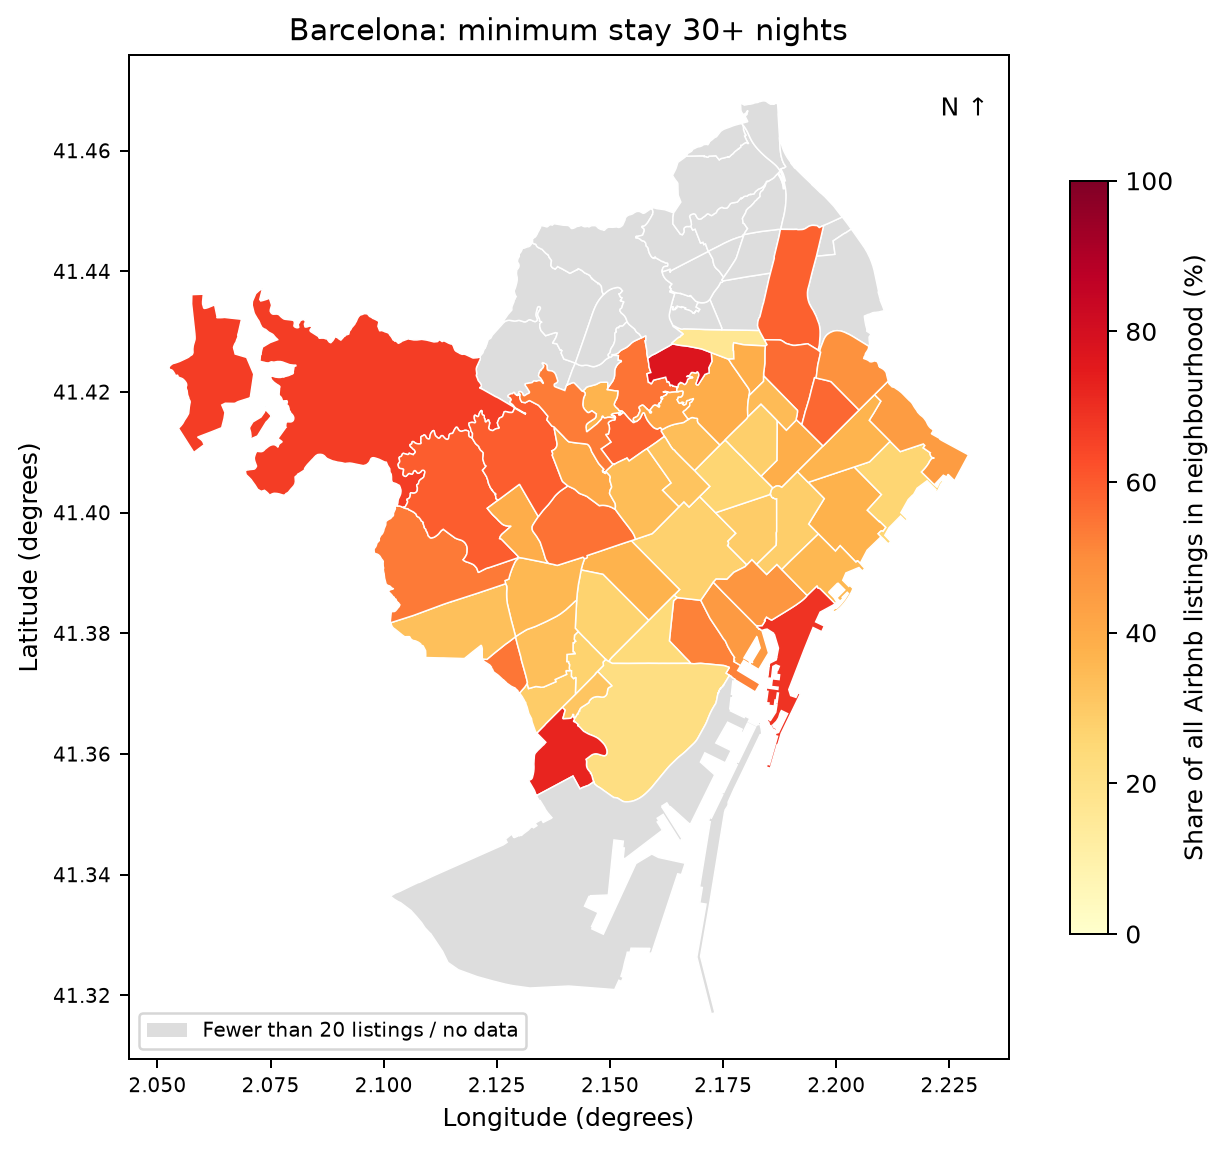
\includegraphics[width=.49\linewidth]{study05_map_monthly_share_barcelona.png}
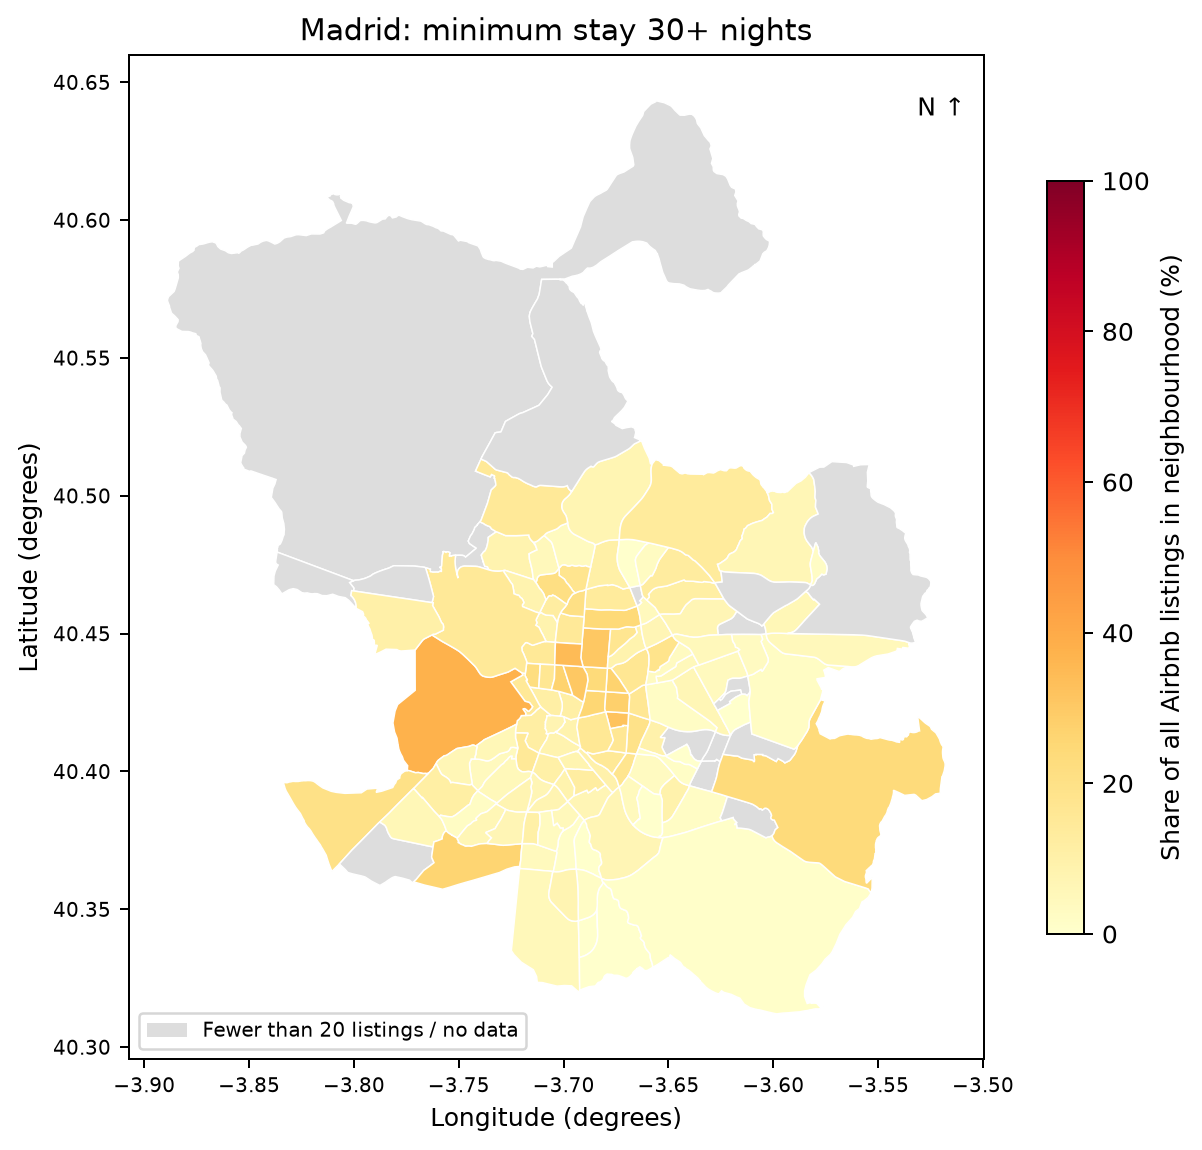
\includegraphics[width=.49\linewidth]{study05_map_monthly_share_madrid.png}
\caption{Static monthly+ neighbourhood shares for the Spanish cities, regenerated with a common 0--100\% scale. Grey means fewer than 20 listings or no data. Six interactive maps additionally provide city-specific legends, three base maps, heat layers, hover details and click popups.}\label{fig:rentalmaps}
\end{figure}
\finding{Monthly+ geography is not simply an outskirts pattern. Barcelona's district shares are 50.9\% in Ciutat Vella and 28.3\% in Eixample. Madrid's Chamber\'i and Salamanca are relatively high (25.6\% and 23.0\%). In Los Angeles, the City of Los Angeles differs from other jurisdictions (74.2\% versus 22.2\% in other cities and 9.2\% in unincorporated areas). These are descriptive boundaries, not an estimated policy effect.}

\clearpage
\section{Study 06: entire homes accepting short stays}
\question{Which neighbourhoods have the largest share of entire-home listings with a minimum stay of 1--29 nights?}

\method{Select entire homes/apartments with advertised minimum stays from 1 through 29 nights. Count segment listings in each neighbourhood and divide by all Airbnb listings in that neighbourhood, including rows with missing prices. This broader short-stay definition includes both the 1--6 and 7--29 categories of study 05.}
\[
\mathrm{share}_{j}=100\times\frac{\#\{\text{entire homes with minimum 1--29 nights in }j\}}{\#\{\text{all Airbnb listings in }j\}}.
\]
\resulttable{short_city}{City totals for the same segment. These are shares of Airbnb listings, not of homes or the housing stock.}{tab:shortcity}
\resulttable{short_top}{The five highest neighbourhood shares in each city among neighbourhoods with at least 20 total listings. Counts make the denominators visible.}{tab:shorttop}
\finding{Barcelona contains \BcnShortN{} qualifying listings (\BcnShortPct{}\% of all listings), and Madrid \MadShortN{} (\MadShortPct{}\%). The highest eligible shares are Vilapicina i la Torre Llobeta in Barcelona (72.2\%, 57 of 79 listings) and Costillares in Madrid (90.0\%, 27 of 30). The latter still has a modest denominator despite passing the threshold. A neighbourhood with a high percentage need not contain the largest absolute number of qualifying listings.}

\textbf{Housing interpretation.} Entire homes with short minimum stays can be used for tourist accommodation, so their spatial distribution is relevant to the housing discussion. These data cannot identify whether individual listings are available, occupied by residents at other times, duplicated across advertisements, or formerly offered as ordinary rentals. We therefore do not call them homes ``taken away'' from residents.
\resulttable{join_audit}{Exact-name joins between listing neighbourhoods and GeoJSON. Every observed neighbourhood matches; areas without listings remain uncoloured.}{tab:joins}
Barcelona has 75 polygon features representing 73 distinct neighbourhood names; one neighbourhood is split into three features. Counts are joined once by name, and its component polygons receive the same value.

\clearpage
\subsection{Static choropleths and join verification}
\begin{figure}[htbp]\centering
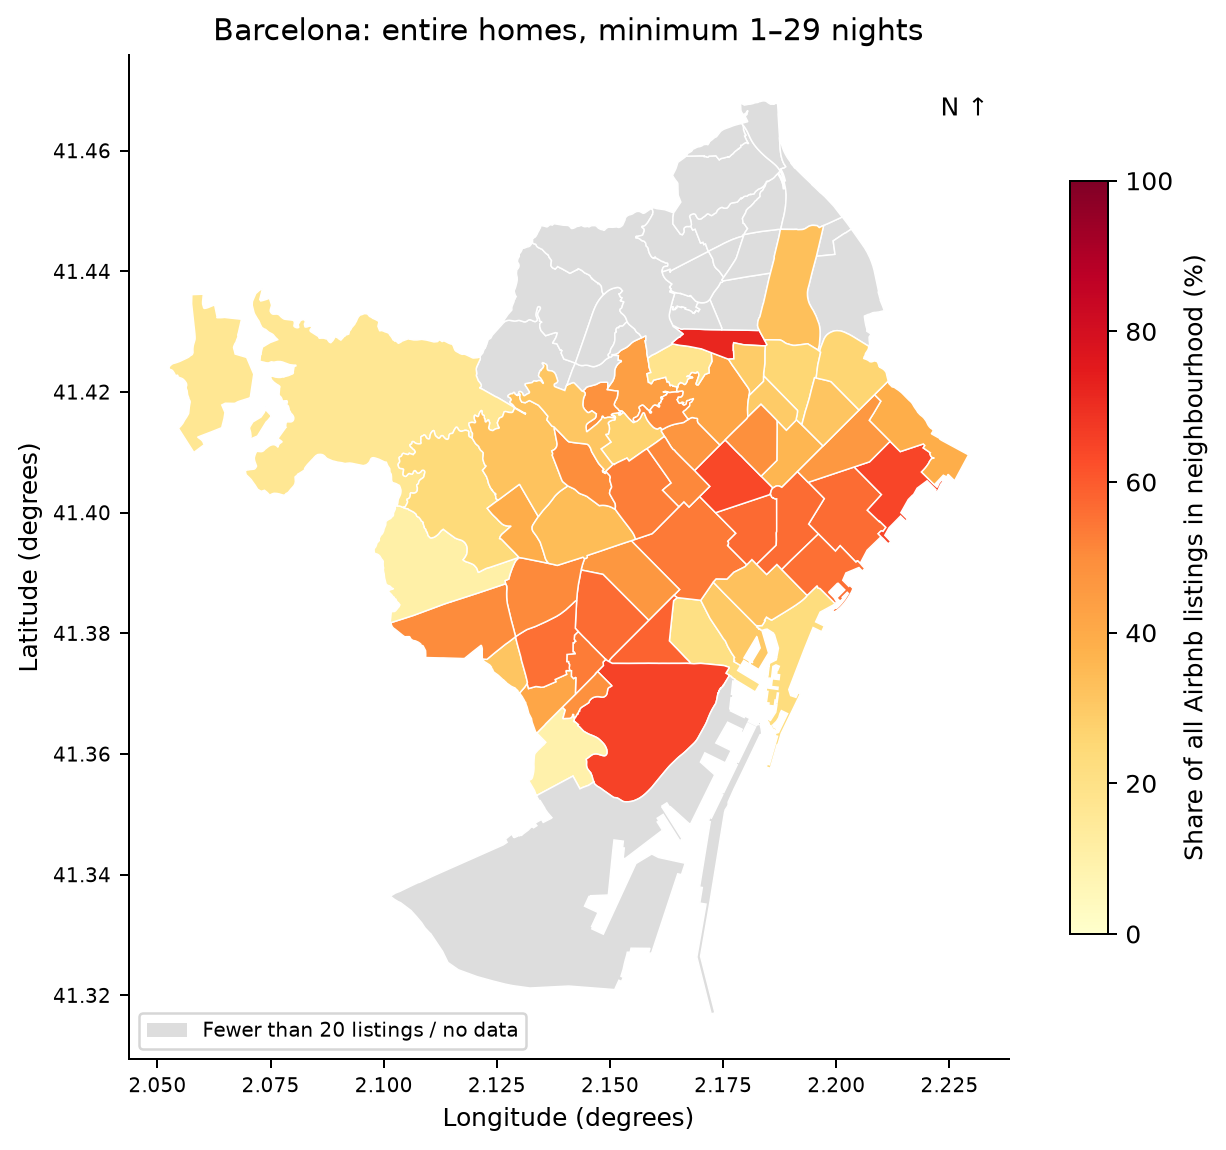
\includegraphics[width=.49\linewidth]{study06_short_entire_barcelona.png}\hfill
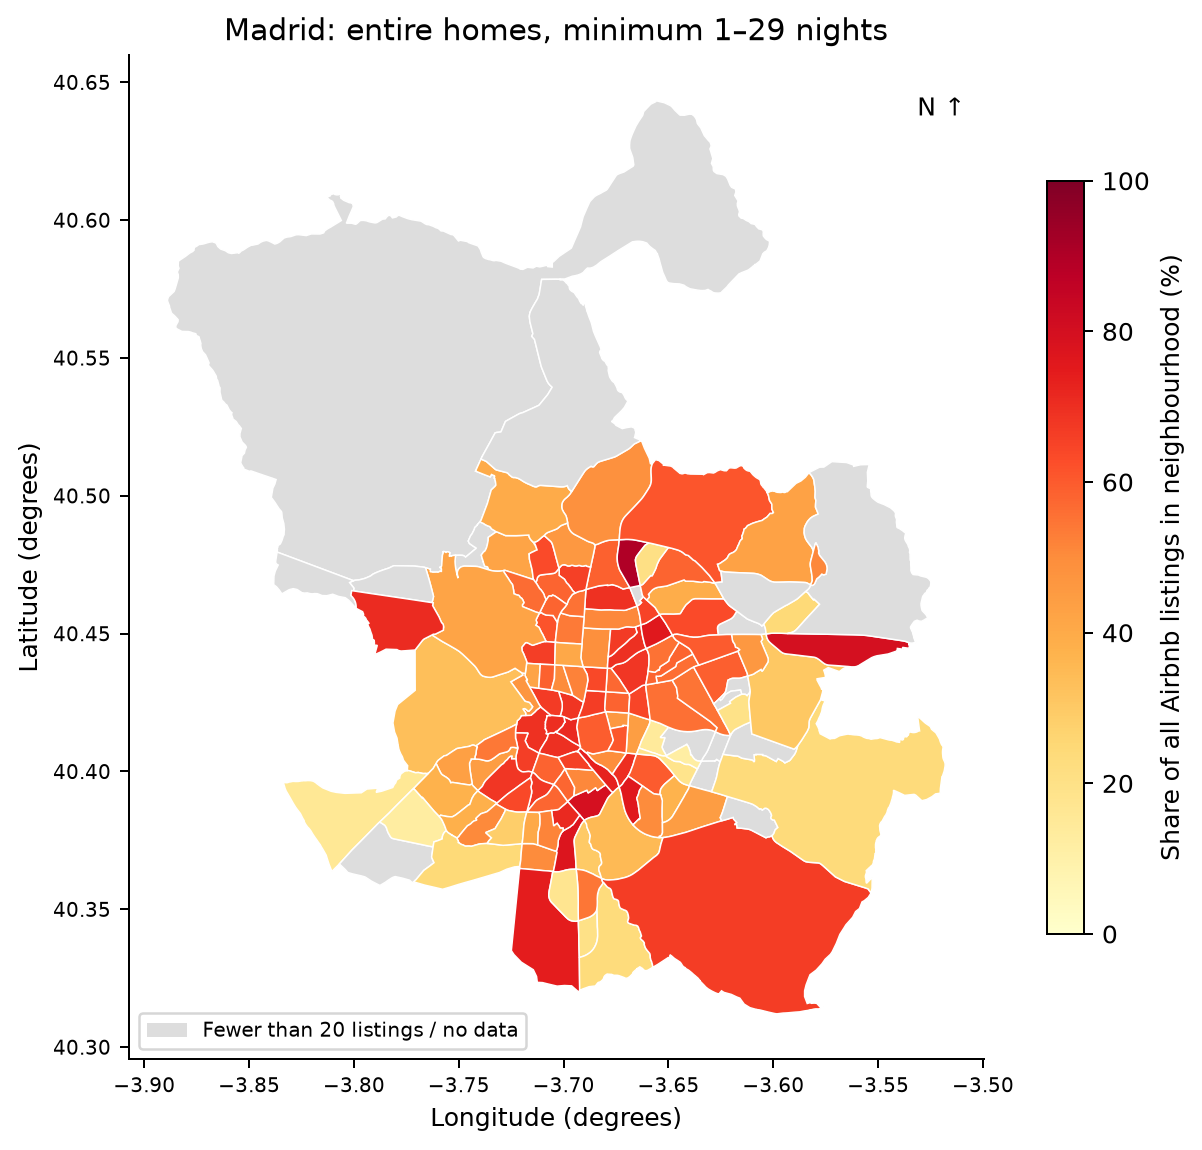
\includegraphics[width=.49\linewidth]{study06_short_entire_madrid.png}
\caption{Entire-home listings with minimum stays of 1--29 nights, as percentages of all neighbourhood Airbnb listings. Left: Barcelona. Right: Madrid. Both maps use the same 0--100\% scale; grey polygons have fewer than 20 listings or no data. Polygon boundaries come from the repository.}\label{fig:shortmaps}
\end{figure}

The static choropleths in Figure~\ref{fig:shortmaps} show the spatial distribution of this segment across city neighbourhoods:
\begin{itemize}
\item In \textbf{Barcelona}, high shares are present in several central and adjacent neighbourhoods, but the highest proportion occurs in Vilapicina i la Torre Llobeta (72.2\%), where entire short-stay homes dominate a relatively modest total supply of 79 listings. Core tourist districts like Ciutat Vella and Eixample have large absolute counts of such listings, but their overall supply is so large that their percentage share is moderate. Peripheral areas with fewer than 20 listings remain uncoloured to prevent small-sample distortion.
\item In \textbf{Madrid}, the highest percentage share is in Costillares (90.0\%, 27 of 30 listings), reflecting a localized pocket of entire-home offers in a small total sample. Central neighbourhoods (such as Sol and Cortes in Centro) exhibit concentrated short-stay entire homes, while outer residential districts generally feature lower shares or fall below the 20-listing threshold.
\end{itemize}
This geographic contrast underscores that proportion-based choropleths must always be read in tandem with absolute supply (Table~\ref{tab:shorttop}) and join verification audits (Table~\ref{tab:joins}).

\clearpage
\section{Study 07: the quoted cost of about one month}
\question{How do normalized monthly-stay quotation costs differ across the two Spanish cities and between entire homes and private rooms?}
\method{Use check-in and checkout dates to compute quote length. Keep 28--35 nights, the two selected room types, positive finite total amounts and a successful EUR quotation in \texttt{price\_quote\_raw}. Calculate $\mathrm{cost}_{30}=\mathrm{quoted\ total}\times30/\mathrm{nights}$. Retain all valid quotes in medians and quartiles.}
\resulttable{monthly_cost}{30-night equivalent quoted amounts. All valid observations enter the statistics; the plot hides outlier points only.}{tab:monthly}
\chart[0.74]{study07_monthly_cost.png}{Normalized quotation costs, split by city and accommodation type. These are not residential rents.}{fig:monthly}
\resulttable{monthly_dates}{Check-in date coverage of the retained quotations. Dates refer to the stay, not the scrape.}{tab:monthlydates}
\finding{Entire-home medians are EUR \BcnEntireMonthly{} in Barcelona (\BcnEntireMonthlyN{} quotes) and EUR \MadEntireMonthly{} in Madrid (\MadEntireMonthlyN{}). Private-room medians are EUR \BcnPrivateMonthly{} (\BcnPrivateMonthlyN{}) and EUR \MadPrivateMonthly{} (\MadPrivateMonthlyN{}). The entire-home medians are close (about 1\% apart), while the private-room median is about 21\% higher in Barcelona. Check-ins span June 2026 to June 2027; the typical entire-home quote starts later in Barcelona (6 August versus 25 July). Different dates and listing composition limit seasonal comparability. The normalized amount is not a newly available 30-night booking, and the source does not establish complete tax and fee coverage. No household-income comparison or affordability conclusion is made.}

\clearpage
\section{Study 08: price and basic listing characteristics}
\question{Does a city price difference remain after accounting for basic accommodation characteristics?}
\method{Estimate one OLS model on complete, valid observations from Barcelona and Madrid:}
\begin{align*}
\log(\mathrm{price})={}&\beta_0+\beta_1\,\mathrm{Madrid}
 +\boldsymbol\gamma^T\mathrm{room\ type}\\
&+\beta_2\log(\mathrm{accommodates})+\beta_3\mathrm{bedrooms}
 +\beta_4\log(1+\mathrm{minimum\ nights})+\varepsilon.
\end{align*}
Barcelona and entire home/apt are the reference categories. Price and capacity must be positive and finite, bedrooms nonnegative, minimum nights at least one, and all included variables observed. No imputation, trimming, extra models or prediction exercise is used. HC3 standard errors allow residual variance to differ across observations.
\resulttable{regression_audit}{Complete-case selection. Missing-price and missing-bedroom counts overlap and must not be added to obtain exclusions.}{tab:regaudit}
\resulttable{regression}{OLS coefficients and 95\% HC3 intervals. The dependent variable is log price. A numerical underflow p-value is reported as a bound.}{tab:reg}
The estimation sample contains \ModelN{} listings. $R^2=\ModelRSq{}$ and adjusted $R^2=\ModelAdjRSq{}$, both on the log-price scale. The design matrix has rank \ModelRank{} out of \ModelCols{} columns and condition number \ModelCondition{}. Coefficients, standard errors and confidence bounds are checked to be finite.

\finding{The Madrid coefficient corresponds to a \CityPct{}\% conditional multiplicative difference from Barcelona, with a 95\% HC3 interval from \CityLow{}\% to \CityHigh{}\%. This is calculated as $100[\exp(\beta_1)-1]$. It is an association in expected log prices, not an arithmetic-mean price effect or a causal city premium. The sample and estimand differ from the unadjusted median comparison in study 03.}

\clearpage
\subsection{Coefficient interpretation and residual diagnostics}
\chart[0.82]{study08_coefficients.png}{Selected OLS coefficients with 95\% HC3 intervals. Continuous coefficients use different units; their raw magnitudes do not rank variable importance.}{fig:coef}
\chart[0.73]{study08_residuals.png}{Residuals versus fitted log prices for every estimation row. Colour represents the number of listings in a bin on a logarithmic scale.}{fig:residual}
The capacity coefficient is an elasticity in the fitted log specification, while the bedrooms coefficient represents one additional bedroom at fixed included covariates. Room-type indicators compare groups conditional on those covariates. Coefficient sizes should be interpreted in their own units.

\finding{The residual distribution and visible extreme errors show the limits of the simple conditional description. HC3 changes uncertainty estimates; it does not remove omitted-variable bias or establish independence. The model omits exact neighbourhood, quotation dates, stay length, amenities and quality, and does not account for shared-host or spatial dependence. Missing bedrooms and prices also select a subset. The model is therefore useful for checking whether the descriptive city difference persists under a small adjustment, not for explaining its causes.}

\clearpage
\section{Study 09: price and guest activity}
\question{Do more expensive entire homes accepting short stays have more reviews from the last year?}
\method{Use the same entire-home, minimum-1--29-night segment as study 06. Require positive finite price and finite, nonnegative annual review counts. Calculate Spearman's rank correlation separately by city, with two-sided p-values. Repeat once for listings whose first review is at least one calendar year before their own scrape date. Ties, including zero review counts, are retained.}
\resulttable{activity}{Spearman correlations between price and reviews in the last twelve months. The established-listing calculation is the only sensitivity check.}{tab:activity}
\chart{study09_price_activity.png}{All eligible observations in both cities; logarithmic price axes improve readability without changing Spearman's ranks. Zero review counts are retained.}{fig:activity}
\finding{The full-sample coefficients are $\rho=\BcnRho{}$ for Barcelona (\BcnActivityN{} listings) and $\rho=\MadRho{}$ for Madrid (\MadActivityN{}). Restricting to listings with at least a year since the first review gives $\rho=\BcnEstablishedRho{}$ and $\rho=\MadEstablishedRho{}$. Barcelona shows a very weak negative relationship, becoming somewhat more negative in the established subset. Madrid is close to zero in both samples, with p-values above 0.05. The results do not support a positive price--activity relationship in these samples.}

Recent reviews are a proxy for guest activity, not occupied nights or realized revenue. A review may follow a long or short stay, many stays are unreviewed, and the first review is not a listing-creation date. The current price can concern a future stay while the review count covers the past year. Location, capacity, quality and pricing responses to demand can confound the association. The age restriction reduces one exposure difference but does not resolve those issues.

\clearpage
\section{Joint conclusions and limitations}
The eight studies describe several distinct dimensions of the platform. Host-account concentration is substantial, but ownership is not observed. Listed prices have long upper tails, and private rooms have lower medians than entire homes across all six cities. Advertised minimum stays divide the cities differently: the monthly+ share is much greater in New York, Los Angeles and Barcelona than in the remaining three cities.

For Barcelona and Madrid, the geography of entire homes accepting 1--29-night minimums identifies neighbourhood differences within Airbnb supply. The city totals are \BcnShortPct{}\% and \MadShortPct{}\%, respectively. These percentages have no residential-housing denominator. They complement the monthly+ maps, but the two segments are not exact complements because the short-stay map restricts room type.

The monthly quotation study describes a selected set of recorded longer-stay offers. Entire-home medians are EUR \BcnEntireMonthly{} and EUR \MadEntireMonthly{} per normalized 30 nights, while private-room medians are EUR \BcnPrivateMonthly{} and EUR \MadPrivateMonthly{}. These amounts cannot be treated as ordinary rents, price-to-income burdens or citywide monthly-market prices. Unequal check-in timing, one quote per listing and uncertain fee coverage are material limitations.

The regression provides a conditional description with $R^2=\ModelRSq{}$ and a Madrid association of \CityPct{}\% relative to Barcelona. It adds information to the raw price comparison but does not isolate a policy or location effect. The price--review correlations of \BcnRho{} and \MadRho{} further show why prices alone cannot stand for realized guest activity or host revenue.

\subsection{Limits shared by the studies}
\begin{itemize}
\item \textbf{Coverage and selection:} these are platform snapshots with missing prices and characteristics, not a complete census of housing or transactions. A listing need not identify one unique dwelling.
\item \textbf{Measurement:} quotations, advertised rules, availability and reviews measure different things over different time windows. None directly supplies actual rents, occupied nights or revenue.
\item \textbf{Comparability:} city boundaries, neighbourhood sizes, accommodation composition, dates and local currencies differ. The cross-currency displays use stated assumptions only.
\item \textbf{Inference:} shared hosts and spatial clustering weaken independent-observation assumptions. Statistical significance does not establish practical importance, representativeness or causality.
\item \textbf{Housing interpretation:} there is no counterfactual use of the dwellings, ordinary-rent series, housing-stock denominator or resident-income data. The project cannot estimate Airbnb's contribution to the housing crisis.
\end{itemize}

The defensible contribution is a transparent, reproducible description of Airbnb offers and their associations, tied to questions relevant to housing discussions while keeping those measurement boundaries explicit.

\clearpage
\section{Reproduction and delivery contents}
The accompanying archive includes the report PDF and LaTeX source, all nine notebooks, shared Python modules, input data, CSV tables, figures and interactive HTML maps. Notebook 01 supplies the initial audit; notebooks 02--09 are the eight studies. No additional data download is required to recompute the analyses.

\subsection{Run the project}
Use Python 3.11 or later and a virtual environment. The tested package versions are recorded in \texttt{requirements-lock.txt}. From the extracted project root on macOS or Linux:
\begin{verbatim}
python3 -m venv .venv
.venv/bin/python -m pip install -r requirements-lock.txt
.venv/bin/python scripts/run_all.py
.venv/bin/python scripts/build_report.py
tectonic --keep-logs report/report.tex
.venv/bin/python scripts/verify_delivery.py
.venv/bin/python scripts/package_delivery.py
\end{verbatim}
On Windows replace \texttt{.venv/bin/python} with \texttt{.venv\textbackslash Scripts\textbackslash python.exe}. A conventional LaTeX installation can compile \texttt{report.tex} twice from the \texttt{report/} directory instead of using Tectonic. Tectonic may need network access on its first run to obtain standard TeX packages. No JupyterLab installation is required; \texttt{nbclient} runs a fresh kernel for each notebook.

\subsection{Outputs and checks}
\begin{itemize}
\item \texttt{tables/}: computed CSV tables, sample-flow audits and notebook execution records.
\item \texttt{figures/}: regenerated statistical plots and static maps used in the report.
\item \texttt{maps/}: existing map images plus exported HTML maps. The six rental-model HTML maps contain choropleths, layer controls, heat maps and popups.
\item \texttt{report/}: editable LaTeX source, generated numerical macros and table fragments, compiled PDF and verification results.
\item \texttt{scripts/}: notebook execution, report-table generation, verification and archive creation.
\end{itemize}
Interactive maps use external basemap services and JavaScript resources, so full browser viewing requires internet access. Static report figures remain usable offline. The retained original screenshots in \texttt{maps/} are supplementary; the report uses reproducibly regenerated figures. A delivery manifest records SHA-256 hashes, and the ZIP is checked for integrity and required paths.

\subsection{Remaining team action}
Replace the title-page author placeholder with the team members' details and recompile before submission. Review the analysis definitions and limitations in preparation for the required interview. The assignment PDFs specify the submission deadline of 25 October 2026 at 23:55 and the interview on 29 October 2026. The report and ZIP are prepared locally; uploading to Campus Virtual is a separate team action.

\clearpage
\begin{thebibliography}{9}
\addcontentsline{toc}{section}{References}
\bibitem{assignment} Universitat Rovira i Virgili. \emph{Pr\`actica 1 -- El poder de les dades: El cas Airbnb}. Sistemes d'Informaci\'o en les Organitzacions, 2026/27. Supplied as \texttt{docs/Enunciat\_P1.pdf}; Polish translation in \texttt{docs/Cw1\_AirBnb.pdf}. These documents define the assignment requirements.
\bibitem{data} Inside Airbnb. \emph{Listing snapshots and neighbourhood boundaries}. Local repository copies for Barcelona, Los Angeles, Madrid, New York, Tokyo and Mexico City; scrape dates in Table~\ref{tab:audit}. Project data portal: \url{https://insideairbnb.com/get-the-data/}. Calculations use the supplied files, not a refreshed download.
\bibitem{bde} Banco de Espa\~na (2024). \emph{Annual Report 2023}, Chapter 4: ``The Spanish housing market: recent changes, risks and affordability problems'', especially the takeaways on p.~210. \href{https://www.bde.es/f/webbe/SES/Secciones/Publicaciones/PublicacionesAnuales/InformesAnuales/23/Files/InfAnual_2023_Cap4_En.pdf}{Official chapter PDF}. Accessed 25 October 2026. Used for brief historical context only.
\bibitem{housing} Consorci de l'Habitatge de Barcelona (25 June 2024). \emph{New measures to tackle the housing emergency and boost available housing}. \href{https://www.consorcihabitatge.barcelona/en/noticies/new-measures-to-tackle-the-housing-emergency-and-boost-available-housing-1414006}{Official announcement}. Accessed 25 October 2026. Cited as an announcement of policy intentions, not an evaluation of outcomes or a statement of current legal status.
\end{thebibliography}
\end{document}
